\documentclass[a4paper,oneside,12pt]{book}

\newcommand{\reporttitle}{Clickstream-based user behavior analytics and recommender system} % Your thesis title
\newcommand{\typeofthesis}{Report}
\newcommand{\authorname}{Your Name} 
%%\newcommand{\authorid}{123456789} 

\newcommand{\department}{Faculty of Information Technology and Electrical Engineering}
\newcommand{\subjectname}{Big Data Processing and Applications}

\AtBeginDocument{
\hypersetup{pdftitle=\reporttitle} 
\hypersetup{pdfauthor=\authorname}
}
\usepackage[T1]{fontenc} 
\usepackage[utf8]{inputenc}
\usepackage[english]{babel}
\addto{\captionsenglish}{%
  \renewcommand{\bibname}{References}
  \renewcommand\thesection{\arabic{section}}
  \renewcommand\thesubsection{\thesection.\arabic{subsection}}
}

\usepackage[a4paper,top=2cm,bottom=2cm,left=2.5cm,right=2.5cm, head=16pt]{geometry}
\setlength{\marginparwidth}{2cm}
\usepackage{adjustbox}
\usepackage{amsmath}
\usepackage{graphicx}
\usepackage{tikz}
\usetikzlibrary{arrows.meta, positioning}
\usepackage[colorlinks=true, allcolors=black]{hyperref}
\usepackage{caption}
\usepackage[parfill]{parskip}
\usepackage{setspace}
\usepackage[numbers,sort&compress]{natbib}
\usepackage{xcolor}
\def\BibTeX{{\rm B\kern-.05em{\sc i\kern-.025em b}\kern-.08em
    T\kern-.1667em\lower.7ex\hbox{E}\kern-.125emX}}
    
\let\Origclearpage\clearpage
\let\clearpage\relax

\usepackage{booktabs}
\usepackage{fancyhdr}

\urlstyle{tt}
\setlength{\emergencystretch}{2em}
\newcommand{\code}[1]{\nolinkurl{#1}}
\usepackage{xurl}
\usepackage{float}

\pagestyle{fancy}
\fancyhf{}
\renewcommand{\headrulewidth}{0pt}
\cfoot{\thepage}
\usepackage{mathpazo}
\usepackage{multirow}
\renewcommand{\theequation}{\arabic{equation}}

\title{\reporttitle}
\author{\authorname}

\begin{document}
\begin{titlepage}
\center



\includegraphics[scale=0.3]{title/unioulu.png}\\[0cm] % FIX: \\[0] -> \\[0cm]


\ifdefined\department
  \Large \textsc{\department} \\[4cm]
  \ifdefined\subjectname
    \large \subjectname\\[1cm]
  \fi



  \textsc{{\huge \bfseries \reporttitle}\vspace{1cm}}\\[1.75cm]


\ifdefined\authorid
\authorname\\ % Your name
\else
\textsc{Nam Do}\\[0.5cm]
\textsc{Leo Davidov}\\[0.5cm]
\textsc{Seyyedhamid Azimidokht}\\[0.5cm]
\textsc{Sajjad Ghaeminejad}\\[2.25cm]
\fi


  \today
\fi

\end{titlepage}
\begin{center}
\fbox{%
\parbox{0.9\textwidth}{%
\centering
\textbf{Live demo:} \url{https://bdpa-clickflow.streamlit.app/}
}}
\end{center}

\vspace{0.5em}
\pagenumbering{arabic}

\section{Project Description}
The increasing availability, volume, and velocity of web log data have motivated data-driven approaches to understand customer behavior and support business decision-making. Large-scale online retailers such as Amazon process tens of millions of transactions daily, not considering auxiliary web interaction data. The key challenge is effectively utilizing these datasets to gain a competitive advantage. Web usage mining has emerged as an important methodology for extracting meaningful patterns from user interactions, resulting in improved personalization, recommendation, and sales optimization.
This project investigates user behavior in an e-commerce setting through clickstream data from an online store \cite{clickstream_data_for_online_shopping_553}. A Big Data pipeline based on Apache Spark is developed to process raw click logs, construct user sessions, and generate features describing user activity.  Our project aims to identify patterns in browsing behavior, analyze relationships between products and user actions, correlations between users, and evaluate the performance of unsupervised learning algorithms in the User-Entity Behavior Analytics setting. In addition, the study evaluates multiple machine learning approaches for recommender systems, and all models are assessed to understand their effectiveness in capturing user preferences.

\section{Related Work}

The authors of the introductory paper to the employed dataset \cite{lapczynski2013discovering} presented several relevant examples. In particular, they referred to the work of Zhang et al. \cite{zhang2007personalised}, whose study focused on the development of a personalized recommendation system. In their experiment, the authors compared the K-means clustering algorithm with a Self-Organizing Map (SOM), also known as a Kohonen map \cite{kohonen1981similarity, kohonen198259}, a type of unsupervised neural network. They constructed sequences of user clicks and grouped them into 20 clusters using both methods, demonstrating that the Kohonen SOM outperformed the classical K-means algorithm.

Another practical example is provided by Carmona et al. \cite{CARMONA201211243}, who analyzed user behavior in an e-commerce environment related to olive oil retail products. In their study, clustering was performed using the K-means algorithm as well, the Apriori algorithm was applied for association rule mining, and the NMEEF-SD algorithm was used for subgroup discovery. The primary objective of subgroup discovery is to identify meaningful patterns in data with respect to a target variable of interest.

As shown in previous studies, clustering algorithms play the dominant role in unsupervised learning related to User-Entity Behavior Analytics (UEBA). This is further supported by the study conducted by Artioli et al. \cite{Artioli2024ACI}, in which 15 clustering methods were evaluated, including variants of K-means, Fuzzy c-means, Gaussian Mixture Models (GMM), DBSCAN, BIRCH, OPTICS, HDBSCAN, SSC-OMP, EnSC, FINCH, SCC, and DenMune. The evaluation was performed on three datasets, including the one used in our project. Among the compared techniques, authors report that BIRCH and DBSCAN provided very promising results when using the dataset employed in this project.

Traditional sequence modeling approaches such as Hidden Markov Models (HMMs) have been widely used in Natural Language Processing science, nevertheless, they are also very applicable in UEBA tasks, for instance, Tynymbayev \cite{TYNYMBAYEV2026200467} used HMM in a cyber-security setting to discover anomalies in log data, he also mentioned that method is much more computationally efficient and of comparable performance with recent approaches which rely on deep learning architectures such as Recurrent Neural Networks (RNNs). In another example Borges et. al \cite{VLMMBorges} measured the ability of a Variable Length Markov Model (VLMM) to summarize user Web navigation sessions up to a given length. On the other side, sequence processing with deep learning has been successfully applied to session-based recommendation tasks \cite{hidasi2016session}, along with transformer-based architectures, which have further improved sequential modeling by leveraging self-attention mechanisms, enabling more effective capture of user behavior patterns in recommendation systems \cite{sun2019bert4rec}, but obviously accounting for more extensive computational requirements.


% Collaborative filtering for implicit feedback forms the foundation of the recommender system. Koren et al.~\cite{koren2009matrix} showed that decomposing the user-item matrix into low-rank latent factors substantially outperforms neighbourhood methods, representing each user $u$ and item $i$ as vectors $\mathbf{p}_u, \mathbf{q}_i \in \mathbb{R}^k$ with predicted interaction $\hat{r}_{ui} = \mathbf{p}_u^\top \mathbf{q}_i$. Hu et al.~\cite{hu2008collaborative} extended this to implicit feedback by converting interaction counts into binary preferences $p_{ui} = \mathbf{1}[r_{ui} > 0]$ with confidence $c_{ui} = 1 + \alpha r_{ui}$. Zhou et al.~\cite{zhou2008largescale} showed that Alternating Least Squares (ALS) solves this objective via independent closed-form updates suitable for distributed execution.

% As a neighbourhood baseline, item-based collaborative filtering~\cite{sarwar2001item} scores candidates by aggregating cosine similarities to items already clicked in the session, exploiting the stability of item co-occurrence patterns without latent factor estimation. Finally, Item2Vec~\cite{barkan2016item2vec} adapts the Word2Vec skip-gram objective~\cite{mikolov2013word2vec} to treat each session as a sentence and each item as a token; candidates are then ranked by cosine similarity to the pooled session embedding.


Recommendation research broadly divides into two families: latent-factor methods, which learn dense user and item embeddings from interaction data, and neighborhood methods, which score candidates by their similarity to items the user has already seen. Both families were significantly shaped at the Netflix Prize (2006-2009) \cite{bennett2007netflix}, a public competition offering \$1\,M for a 10\% improvement over Netflix's own algorithm that produced several of the foundational results used in this project.

On the latent-factor side, Koren, Bell, and Volinsky \cite{koren2009matrix} showed that decomposing the user-item interaction matrix into low-rank user and item
embeddings substantially outperforms neighbourhood-based methods on the Netflix
Prize benchmark, though their formulation requires explicit ratings that clickstream data does not provide. Hu, Koren, and Volinsky \cite{hu2008collaborative} addressed
this by adapting matrix factorization to implicit feedback, weighting each observed
interaction by a confidence score $c_{ui} = 1 + \alpha r_{ui}$ rather than treating
it as a direct preference. Zhou et al. \cite{zhou2008largescale} showed that
Alternating Least Squares (ALS) solves this objective efficiently at scale through
parallelizable factor updates, which Spark MLlib already provides for the distributed implementation. On the neighborhood side, Linden, Smith, and York \cite{linden2003amazon} demonstrated the approach at industrial scale in Amazon's recommendation system, where a pre-computed item-item similarity matrix enables near-instantaneous scoring with every suggestion traceable to a specific item in user's history. Sarwar
et al. \cite{sarwar2001item} established that this item-based formulation is competitive with model-based methods on sparse implicit-feedback data while being far more interpretable. Pazzani and Billsus \cite{pazzani2007content} further note it generalises to content features when interaction signal is thin. We adopt the co-interaction variant along side ALS, enabling a direct comparison of global latent-factor structure against local item-item similarity on identical evaluation data.

\section{Data Description}

The dataset is the \textit{Clickstream Data for Online Shopping} from the UCI ML Repository \cite{clickstream_data_for_online_shopping_553}, originally introduced in \cite{lapczynski2013discovering} and licensed CC BY 4.0. It contains 165,474 clicks over 24,026 sessions from an online clothing store, collected April--August 2008, with no missing values. It is a semicolon-delimited CSV with 14 fields (Table \ref{table:data_description}).

\begin{table}[H]
\footnotesize
\caption{Dataset field descriptions}
\label{table:data_description}
\begin{adjustbox}{center,width=1.1\textwidth,center=\textwidth}
    \begin{tabular}{p{3.8cm}p{6.5cm}p{1.2cm}p{1.8cm}}
    \toprule
         Field name & Description & Type & Example \\
         \midrule
         order & Click index within a session & integer & 1 \\
         country & Country code (47 values) & integer & 29 \\
         session\_id & Session identifier & integer & 1 \\
         page\_1\_main\_category  & trousers (1), skirts (2), blouses (3), sale (4) & string & ``2'' \\
         page\_2\_clothing\_model & Product code (217 models) & string & ``A13'' \\
         colour & Product colour (14 categories) & string & ``2'' \\
         location & Photo position (6 zones) & string & ``5'' \\
         model\_photography & en face (1) or profile (2) & string & ``1'' \\
         price & Price in USD & integer & 28 \\
         price\_2 & Price exceeds category average & boolean & false \\
         page & Page within the store (1--5) & integer & 1 \\
         date & Click date (merged from y/m/d) & date & 2008-04-01 \\
    \bottomrule
    \end{tabular}
\end{adjustbox}
\end{table}

Clicks are evenly spread across categories (trousers 30.1\%, skirts 23.2\%, blouses 23.3\%, sale 23.4\%) and the \texttt{price\_2} flag is balanced (51.2\% above-average). Prices range 18--82 USD (mean 43.80). Sessions average 6.89 clicks with standard deviation 8.99 and maximum 195, indicating a strong right skew. 

All preprocessing steps and feature engineering methods were tailored to the analysis and machine learning methods, depending on the experiment, such as groupings, date conversion/expansion, or weekday derivation. 

\section{Methods and Tools}

\subsection{User-Entity Behavior Modeling}

\subsubsection{Event-Level}

For the experimental setup, we selected \textbf{Gaussian Mixture Model (GMM)}, \textbf{K-Means}, and a hierarchical variant, \textbf{Bisecting K-Means}. K-Means-based methods are widely used in UEBA and recommender systems because they are simple and efficient on medium-sized datasets. The bisecting variant can be less sensitive to centroid initialization, as it recursively splits clusters into smaller partitions. GMM, in contrast, fits the data to a predefined number of multivariate Gaussian distributions, and each sample is represented as a mixture of membership probabilities, which allows GMM to model overlapping clusters through soft assignment. K-Means, by comparison, is a distance-based method that performs hard assignment. 

Our clickstream data is dominantly categorical, making dimensionality reduction an important consideration. Applying One-Hot Encoding directly results in high-dimensional (300+), sparse feature vectors. This sparsity negatively impacts algorithms such as K-Means relying on Euclidean distance, since this metric vanishes in high-dimensional spaces. \textbf{Principal Component Analysis (PCA)} is a widely used dimensionality reduction technique, but it is not naturally well-suited for categorical data, as it assumes continuous variables. Nevertheless, Datta et al. \cite{datta} report better performance when combining K-Means with PCA, in contrast to Artioli et al. \cite{Artioli2024ACI}, who instead applied standard scaling to categorical features. In our approach, we adopt a hybrid strategy that combines elements of both methods. Specifically, we apply standard scaling to \textit{price}, and additionally transform the \textit{page 2 (clothing model)} feature by splitting it into its alphabetical and numerical components, as well as perform grouping of \textit{country} before applying PCA.

The final model and feature set are selected based on clustering performance metrics, including the Silhouette score, Davies-Bouldin index, and Calinski-Harabasz score.

\subsubsection{Session-Level}

Session-level clustering differs fundamentally from raw event-level clustering, as the order of user interactions matters, in addition to the overall mixture of those interactions within each session. In this context, each unique click in the dataset can be treated as a token.

To model the content of sessions, we employ \textbf{Latent Dirichlet Allocation (LDA)} \cite{lda}, a probabilistic Bayesian method that represents each session as a mixture of latent topics, where each topic corresponds to a distribution over click-tokens. This specific formulation allows us to capture the click co-occurrence patterns within sessions and facilitates the discovery of latent behavioral patterns through topic mixtures. LDA follows aka "bag-of-clicks" assumption in this form and does not explicitly account for temporal order, though it can be achieved by employing n-grams of clicks.

Classical approaches, such as Markov models, can represent user navigation as transitions between states, effectively modeling short sequences, whereas modern methods, including RNNs and Transformer models, can learn complex sequential patterns and long-range dependencies, so we additionally employ an intermediate approach by considering \textbf{Word2Vec} \cite{mikolov2013word2vec}, which can be used to learn dense vector representations of user clicks represented as unique tokens based on their co-occurrence within local context windows. While it does not explicitly model full sequences like RNNs or Transformers, it can capture contextual similarity between clicks more effectively than LDA and produces continuous embeddings that are well-suited for tasks such as clustering, UEBA, and recommender systems. Session representations are obtained via context pooling, implemented as the normalized sum of click embeddings. In addition, we evaluate the normalized TF-IDF \cite{SALTON1988513} representation of user sessions. 

For clustering, we employ K-Means and Bisecting K-Means with cosine distance for both TF-IDF and Word2Vec-based representations. Optimal parameter search is based on the same metrics as in event-level experiments, while LDA is evaluated using log-likelihood and perplexity, where higher log-likelihood and lower perplexity indicate better model fit.


%  (Nam): add method and tool for recommender system (DONE)


% \subsection{Recommender System}
% \subsubsection{Experimental Setup}
% Sessions whose first click falls in months 4--7 form the training set, and
% sessions whose first click falls in month 8 form the test set, giving a strict
% temporal split that prevents future data from leaking into training.
% Within each test session the final click is held out as the ground truth item;
% all preceding clicks are available as session context.
% Test sessions are further partitioned into \textit{warm} sessions, which have
% at least two context clicks after removing the ground truth, and \textit{cold}
% sessions, which have exactly one context click.
% All models exclude items already seen in the session context before scoring
% candidates, and all recommendation lists are truncated to $K = 10$.

% \subsubsection{Baseline}

% The popularity ranker scores every candidate item by its total click count in
% the training set, removes items the session has already seen, and returns the
% top-10 most clicked items.
% It carries no personalisation and serves as the lower bound against which all
% other models are compared.

% \subsubsection{Alternating Least Squares}

% ALS is trained on the session-item interaction matrix constructed from training
% sessions, where each entry is the raw click count for a (session, item) pair.
% We use the implicit feedback formulation of Hu et al.~\cite{hu2008collaborative},
% with confidence parameter $\alpha = 80$, latent rank $k = 20$, regularisation
% $\lambda = 0.1$, and 15 iterations.
% The model is fitted using the distributed ALS implementation in Spark
% MLlib.
% Because test sessions are unseen during training, their latent vectors are
% estimated at inference time via a fold-in step: given the context clicks of a
% test session, a closed-form least-squares update is solved against the frozen
% item factor matrix to produce a temporary session vector, which is then scored
% against all 217 item vectors by dot product.

% \subsubsection{Item $k$-Nearest Neighbours}

% Item vectors are constructed from the session-item interaction matrix and
% L2-normalised column-wise, so that each item is represented by its normalised
% co-occurrence profile across sessions.
% Cosine similarity between every pair of items is computed via a distributed
% self-join on the normalised matrix, and the top-50 most similar neighbours are
% retained per seed item.
% Recommendations for a target session are produced by taking each item in the
% session context as a seed, retrieving its neighbours, and accumulating weighted
% similarity scores across all seeds, with ties broken by item index.

% \subsubsection{Item2Vec}

% Item embeddings are trained with PySpark MLlib's Word2Vec implementation using
% the skip-gram objective, treating each ordered session as a sentence and each
% product code as a token.
% Hyperparameters are: \texttt{vectorSize}$=32$, \texttt{windowSize}$=5$,
% \texttt{maxIter}$=20$, \texttt{minCount}$=1$.
% At inference time a session vector is computed by exponentially weighted
% pooling of the context item embeddings with decay $\gamma = 0.8$, assigning
% weight $\gamma^{n-t}$ to the click at position $t$ in a session of length $n$,
% so that more recent clicks contribute more to the session representation.
% Candidate items are then ranked by cosine similarity to this session vector.

% \subsubsection{Sequential Warm-Up for Cold Sessions}

% Cold sessions have a single context click, which is too little signal for
% ALS fold-in or Item2Vec pooling to be effective.
% For these sessions we apply a first-order Markov transition model trained on
% all consecutive item pairs in the training set.
% Given the single observed item, the model scores every candidate by the
% empirical transition probability from that item and returns the top-10
% transitions.

% \subsubsection{Evaluation Metrics}

% All models are evaluated on the test set using four metrics computed at $K=10$.

% \begin{itemize}
%     \item \textbf{MRR@10}: mean reciprocal rank of the held-out ground truth
%           item across test sessions. It rewards models that rank the correct
%           item higher in the list.

%     \item \textbf{Recall@10}: fraction of test sessions in which the held-out
%           item appears anywhere in the top-10 list.

%     \item \textbf{Coverage}: share of the 217-item catalogue that appears in
%           at least one top-10 list across all test sessions. Low coverage
%           indicates the model concentrates recommendations on a small subset
%           of popular items.

%     \item \textbf{Novelty@10}: mean self-information of recommended items,
%           defined as
%           \[
%               \text{Novelty} = \frac{1}{|S|} \sum_{s \in S}
%               \frac{1}{K} \sum_{i \in \hat{L}_s}
%               -\log_2 p(i),
%           \]
%           where $p(i)$ is the relative click frequency of item $i$ in the
%           training set and $\hat{L}_s$ is the top-10 list for session $s$.
%           Higher novelty indicates the model surfaces less obvious items.
% \end{itemize}

\subsection{Recommender System}

\subsubsection{Experimental Setup}

Sessions from months 4--6 form the training set and sessions from months
7--8 form the test set, giving a strict temporal split.
Within each test session the final click is held out as the ground truth, and sessions with no remaining context are excluded.
Test sessions are split into two tracks based on context length: \textit{warm}
sessions have at least two context clicks ($n = 2{,}265$), and \textit{cold}
sessions have exactly one context click ($n = 3{,}320$), accounting for
47.5\% of the test pool and reflecting the prevalence of short sessions in
the data. All models exclude items already seen in the session before ranking, and
lists are truncated to $K = 10$. As a comparison baseline, we use a popularity ranker as the lower bound in both \textit{warm} and \textit{cold} session tracks. It scores every candidate by its total training-set click count and returns the top-10 most popular items, ignoring session context entirely.

\subsubsection{Warm Sessions}

Three models are evaluated on warm sessions, where enough context is
available to estimate session preferences.

\textbf{Alternating Least Squares (ALS).}
ALS is trained on the session--item click-count matrix using the implicit
feedback formulation of Hu et al.~\cite{hu2008collaborative}, which
replaces raw counts with confidence weights ($c_{ui} = 1 + \alpha r_{ui}$)
rather than treating clicks as explicit ratings.
This makes it the natural choice for clickstream data.
Spark MLlib's distributed ALS implementation is used directly, with
$\alpha = 80$, rank $k = 20$, regularisation $\lambda = 0.1$, and 15
iterations.
Because test sessions are unseen at training time, their latent vectors are
estimated at inference via a fold-in step: a closed-form least-squares
update against the frozen item factor matrix produces a temporary session
vector, which is then scored against all 217 items by dot product.

\textbf{Item $k$-Nearest Neighbours (Item k-NN).}
Item k-NN scores candidates by co-occurrence rather than latent factors,
following the item-based formulation of Sarwar et al.~\cite{sarwar2001item}.
It is included as a transparent neighbourhood baseline: every
recommendation is traceable to a specific item in the session context,
enabling a direct comparison of local item similarity against global
latent-factor structure. Each item is represented by its L2-normalised co-occurrence profile across sessions, and the top-50 nearest neighbours per item are retained via
distributed cosine self-join. Candidate scores are accumulated across all context items and ranked.

%\textbf{Item2Vec.}
%Item2Vec captures order-sensitive co-occurrence patterns that aggregate
%click counts cannot express~\cite{mikolov2013word2vec}.
%Each session is treated as a sentence and each product code as a token;
%the skip-gram objective trains 32-dimensional item embeddings
%(\texttt{windowSize}$=5$, \texttt{maxIter}$=20$, \texttt{minCount}$=1$)
%using PySpark MLlib's Word2Vec.
%At inference, a session vector is formed by exponentially weighted pooling
%with decay $\gamma = 0.8$, giving more weight to recent clicks, and
%andidates are ranked by cosine similarity to this vector.

\textbf{Item2Vec.}
Additionally, we evaluate Item2Vec, a Word2Vec derivative in the context of recommendation systems, which was initially proposed by Barkan et al. \cite{barkan2016item2vec}, and, as in the session-level modeling, user sessions are treated as sentences, while clicks on unique products in the catalog are treated as tokens. At inference, we modify user context pooling by injecting temporal aspect via the exponentially weighted mean (EWM) of item embeddings based on the reverse interaction order with a weighting factor formulated as $\gamma^{\Delta t}$, giving more attention to recent interactions with a smaller $\gamma$. Recommendation candidates are ranked by cosine similarity to the resulting vector. The optimal parameters for the Word2Vec are based on the session-level clustering performance, while decay $\gamma$, is separately optimized.

\subsubsection{Cold Sessions}

Cold sessions provide only one context click, which is too little signal
for ALS fold-in and Item2Vec session context pooling via EWM.
A first-order \textbf{Markov transition model} is used instead: it scores
every candidate by the empirical probability of transitioning to that item
immediately after the observed click in the training set.
No latent factors or embeddings are needed only a frequency count over
consecutive item pairs -- yet the model is already more personalised than
global popularity because it conditions on the specific observed item.

\subsubsection{Evaluation Metrics}

All models are evaluated at $K = 10$ using four metrics that jointly cover
accuracy and catalogue diversity.

\begin{itemize}
    \item \textbf{MRR@10}: mean reciprocal rank of the ground truth item.
          Rewards models that rank the correct item higher.

    \item \textbf{Recall@10}: fraction of sessions where the ground truth
          appears in the top-10 list.

    \item \textbf{Coverage}: share of the 217-item catalogue appearing in
          at least one top-10 list. Low coverage indicates over-concentration
          on popular items.

    \item \textbf{Novelty@10}: mean self-information of recommended items,
          $\frac{1}{|S|K}\sum_{s}\sum_{i \in \hat{L}_s} {-\log_2 p(i)}$,
          where $p(i)$ is the relative training-set click frequency of item
          $i$. Higher values indicate less obvious recommendations.
\end{itemize}

% TODO (Hamid): add tools and motivation for EDA 
% TODO (Leo): add tools and motivation for ML

\section{Data Analysis}
\subsection{Exploratory Data Analysis}

The EDA focused on identifying behavioural patterns that are directly useful for the later modelling and recommendation stages. The first important observation is that browsing behaviour is geographically concentrated. Poland is by far the dominant segment, while Other EU is the second largest group. This means that the most reliable behavioural conclusions come from the Polish segment, and results for smaller regions should be interpreted more cautiously. Category-level behaviour shows both overall popularity and regional variation. Trousers are the most viewed category overall, followed by sale, blouses, and skirts. However, the regional breakdown is more informative than the global ranking. In Poland, sale items are almost as frequent as trousers, while in Other EU, trousers and blouses dominate more clearly. This suggests that a single global view of product interest can hide regional differences that may be useful for personalization. 

At the product level, the most viewed clothing models are B4, A2, A11, P1, and B10. These products form a natural popularity baseline: a simple recommender can suggest the most-clicked items to all users. However, the product frequency distribution is long-tailed, meaning that a small set of products receives a large share of the clicks while many products receive limited attention. This supports the need to evaluate recommender systems not only by accuracy, but also by coverage, since a popularity-only approach may ignore long-tail items. Colour preference gives another interpretable signal. Black and blue are the two dominant colours overall. The same colours are also prominent across regions, although their ordering differs slightly. This indicates that colour can be useful as an explanatory product attribute and as a potential feature for personalization or catalogue analysis. The strongest behavioural insight for the modelling stage is that sessions are short. The median session contains only four clicks, and 39.6\% of sessions stop on the first page. This confirms that many users provide only a short interaction history. Therefore, recommendation methods need to work early in the session, which supports the use of item-to-item co-interaction methods and cold-session strategies. 

Finally, association analysis was used to connect EDA with the association-rule and item-based recommendation methods discussed in the related work. In this analysis, support measures how frequently two categories or products appear together among all sessions, confidence measures how often the consequent appears when the antecedent is present, and lift compares the observed co-occurrence against what would be expected by chance. For example, at the category level, the Polish rule blouses $\rightarrow$ trousers has support 0.23, confidence 0.54, and lift 1.03. This means that 23.34\% of Polish sessions contain both blouses and trousers, 53.91\% of blouse sessions also contain trousers, and the pair appears together 1.03 times more often than expected under independence. Product-level rules show stronger associations: for example, B10--B13 has lift 4.67, and A2--A3 has lift 4.986. These co-view patterns provide interpretable evidence for item-based recommendation, because they show which products tend to appear together within sessions.

\subsection{Event-Level Experiments}

Our experiments focused on multiple feature configurations, directed to the temporal aspect of the data, in addition to the strategy mentioned in the methodology section, we included cyclic encoding of \textit{day} (or derived weekday) using sine and cosine transformations, linear scaling of \textit{day}, inclusion or exclusion of OHE-encoded \textit{month}, and complete removal of temporal features before PCA.

\begin{figure}[H]
\centering
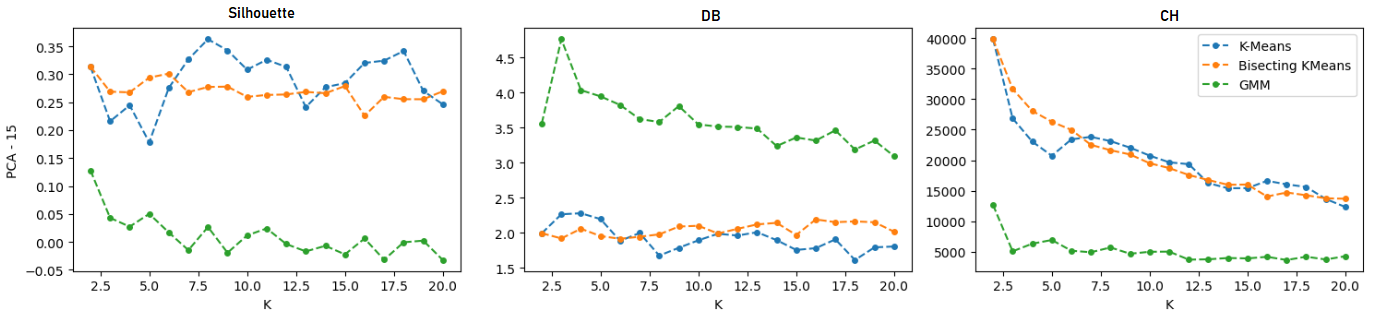
\includegraphics[width=1\linewidth]{best_event_level.png}
\caption{Experiment 2}
\label{experiment 2}
\end{figure}

Different numbers of principal components (30, 20, 15) were evaluated, corresponding to explained variance levels of approximately 90\%, 83.5\%, and 75\%, respectively. The best performance was achieved in Experiment 2, shown in Figure \ref{experiment 2}, using 15 components without temporal features. K-means consistently outperformed Bisecting K-Means and GMM in all setups, achieving the highest silhouette scores up to 0.36 for larger values of K, as well as the lowest Davies–Bouldin values, and Calinski–Harabasz scores $\sim$ 20–40k, with best performance at K = 8 in Experiment 2. The bisecting variant showed slightly better result only for smaller numbers of clusters, while GMM performed poorly overall, with near-zero or negative silhouette scores and high Davies–Bouldin values, indicating significantly overlapping clusters. The inclusion of temporal features reduced clustering quality, while higher-dimensional representations required larger values of K across all configurations, suggesting over-segmentation and the introduction of noise. These results indicate that temporal features do not provide a meaningful signal in this setting, and that simpler feature representations combined with K-Means yield the most effective clustering structure.

\subsection{Session-Level Experiments}

For tokenization, we excluded all temporal features and \textit{country}. It appeared that the dataset has only 218 unique click feature combinations, which are basically completely described by \textit{page 2 (clothing model)}. We experimented with encoding regional groupings, but it didn't yield any improvements, as most of the logs are coming from Poland. We do not explicitly present figures for the TF-IDF representation, as this setup resulted in the poorest performance, yielding a cosine silhouette score of $\sim0.09$ even at K = 20 for both K-Means variants. This is likely due to the high sparsity of the resulting vectors. In contrast, session context vector pooling using Word2Vec embeddings produced the performance results presented below.
\begin{figure}[H]
\centering
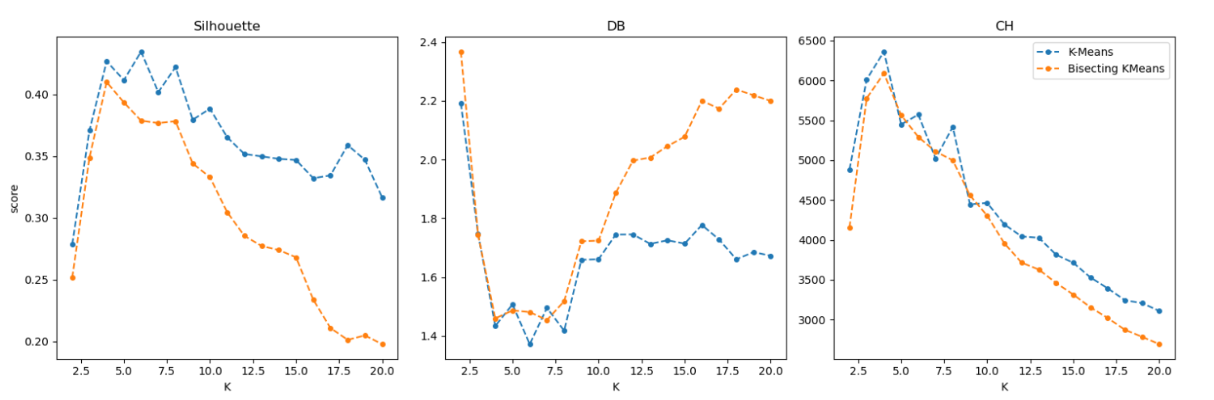
\includegraphics[width=1\linewidth, height=0.15\textheight]{w2v.png}
\caption{Session Context Vector Clustering}
\label{w2v}
\end{figure}
\begin{figure}[H]
\centering
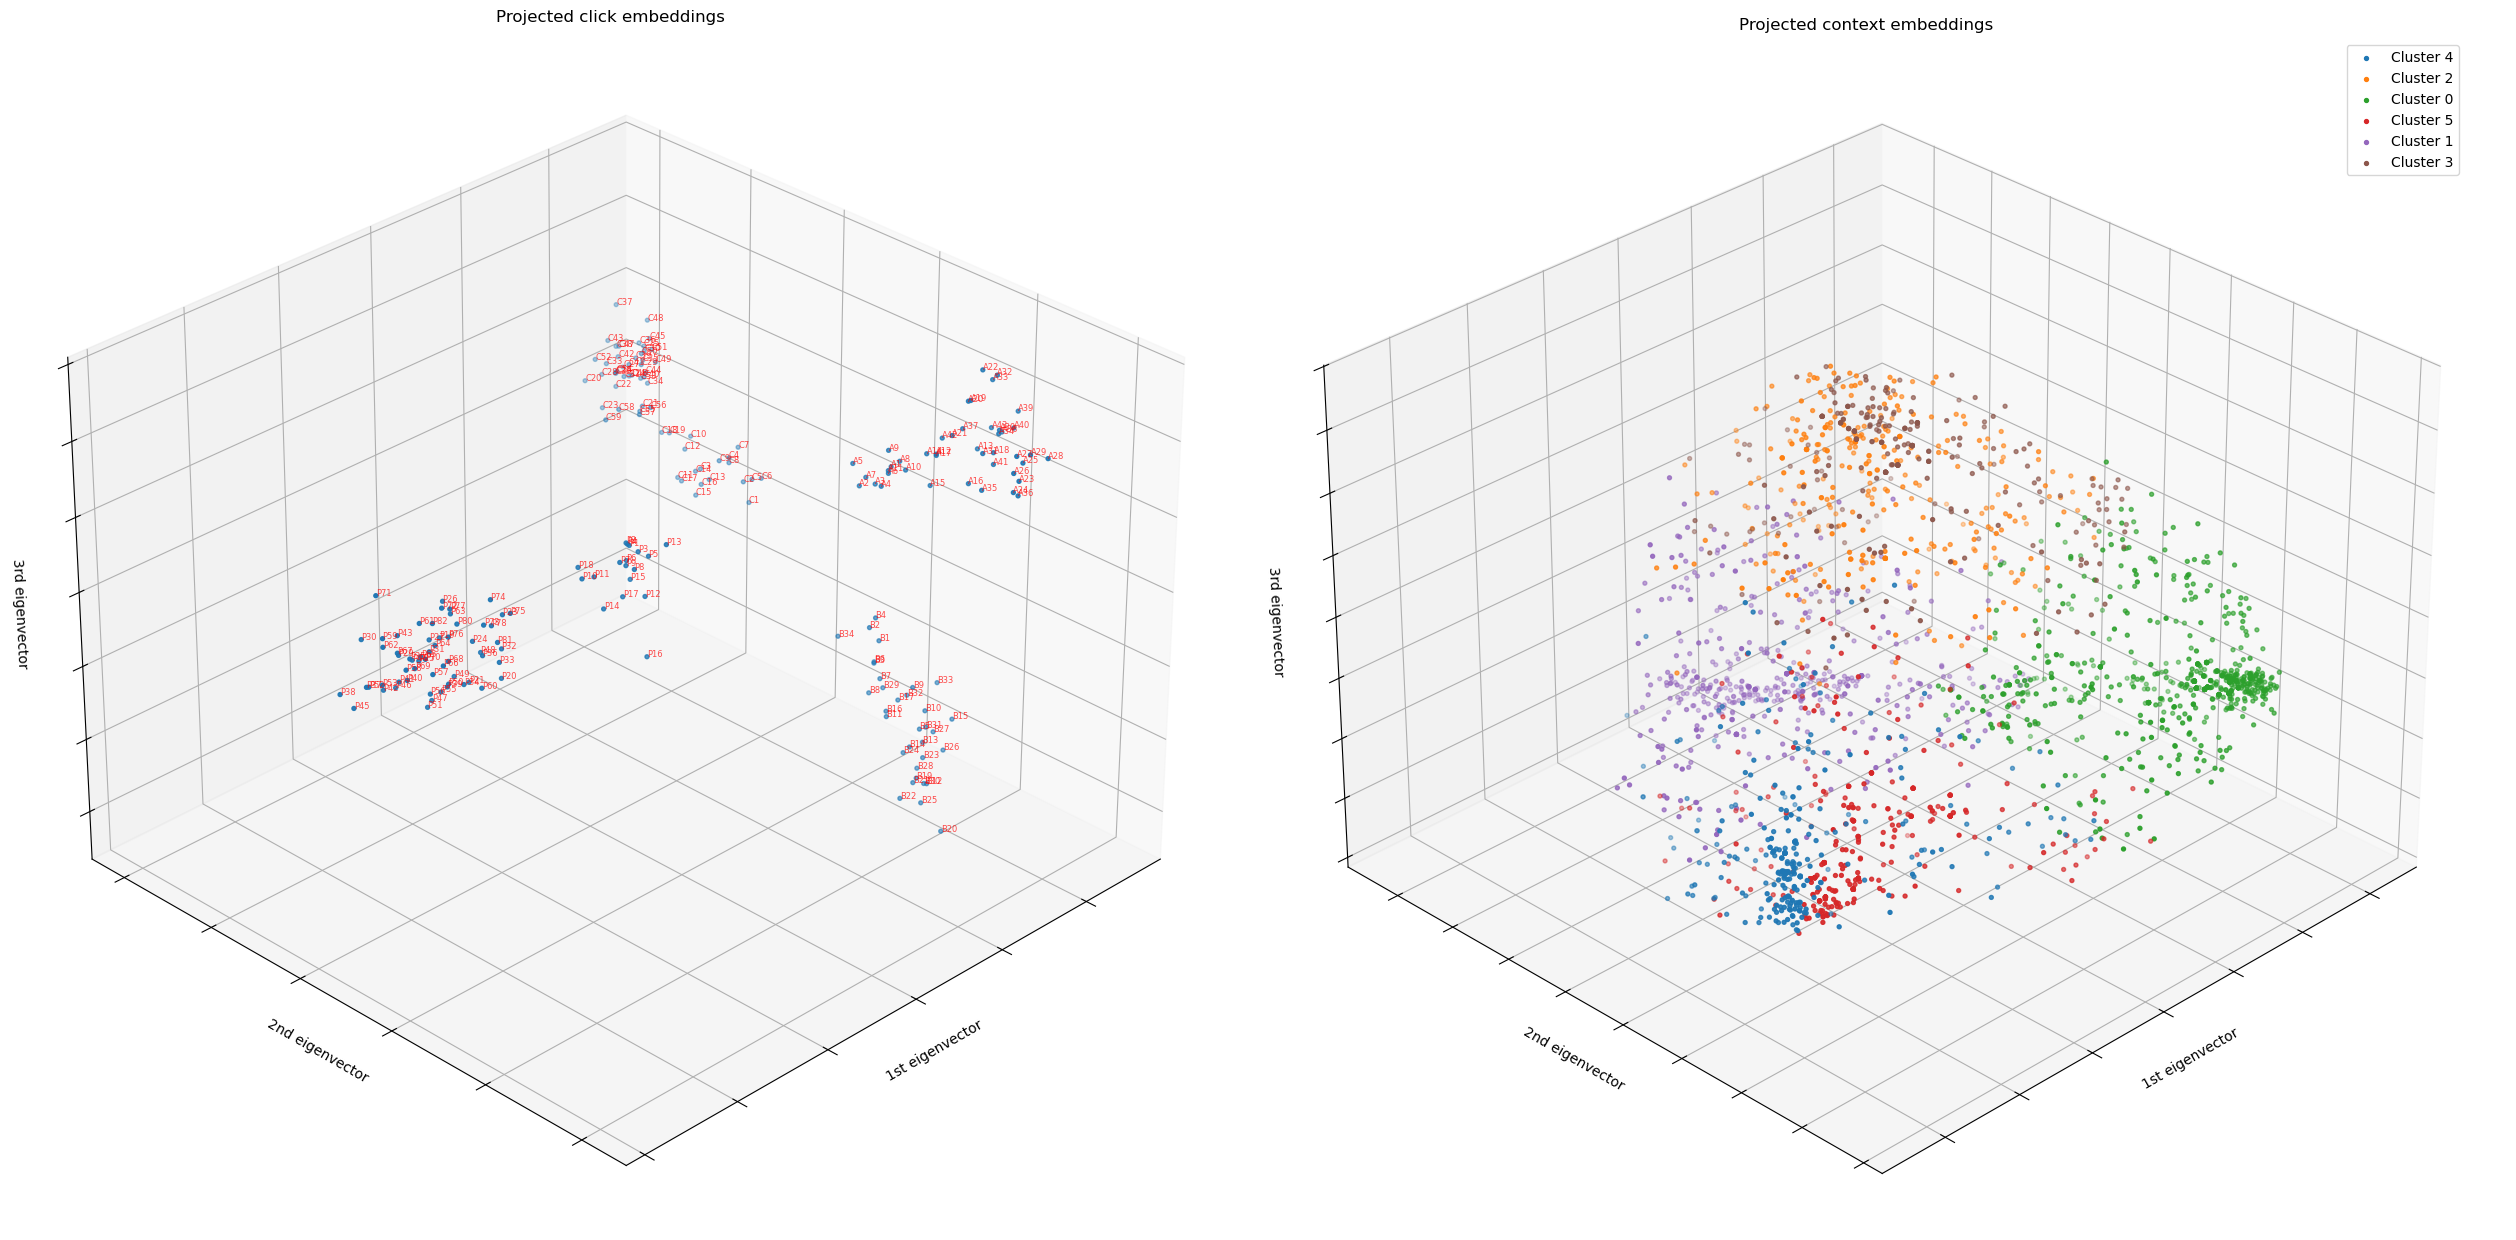
\includegraphics[width=0.7\linewidth]{clusters_embeddings.png}
\caption{Click embeddings (Left) and Clusters of Pooled Context Vectors (Right)}
\label{emdeddings}
\end{figure}
The quality of embeddings was evaluated with window sizes of 3-5, as sessions on average have a length of 7 and a median of 4, producing similar results for both windows. The minimum token frequency was set to 5, ignoring rare page clicks that do not provide enough context for training, and the embedding dimension was set to 32. The resulting vocabulary yielded a vectorization of 213 click tokens. For topic modeling with LDA, default parameters were used. The best performance for LDA was observed at K = 4, with perplexity = 4.919 and log-likelihood = $-8.14 \times10^{5}$. The best number of topics is well aligned with the number of product categories. In contrast, the context vector representation of sessions using Word2Vec embeddings in our setup achieved peak results at K = 6 as shown in the Figure \ref{w2v}, reaching a cosine silhouette score of $\sim0.43$, Davies–Bouldin index < 1.4, and Calinski–Harabasz score > 6k. These results indicate a consistent cluster structure, where 32-dimensional session context vectors effectively capture similarities in user browsing patterns. Representative examples of click-embedding clouds and clusters of user browsing contexts projected into 3D using PCA are presented in Figure \ref{emdeddings}.

% \subsection{Recommender System}

% Sessions are split temporally: months 4--6 form the training set (17,031
% sessions) and months 7--8 form the test set (6,995 sessions).
% Within each test session the final click is held out as the ground truth;
% sessions with no remaining context clicks are excluded, leaving 5,585
% evaluable test sessions.
% Test sessions are partitioned into warm sessions ($\geq 2$ context clicks,
% $n = 5{,}585$), evaluated by ALS, item k-NN, and Item2Vec, and cold sessions
% ($= 1$ context click, $n = 3{,}320$), evaluated by the sequential warm-up
% model.
% Cold sessions account for 47.5\% of the total test pool, reflecting the
% prevalence of short sessions in the data and motivating separate evaluation
% tracks for the two groups.
% Table~\ref{tab:recommender_split} summarises the data partition.

% \begin{table}[H]
% \centering
% \caption{Recommender train/test split summary}
% \label{tab:recommender_split}
% \begin{tabular}{lrrl}
% \hline
% Split                  & Sessions & Months & Evaluated by \\
% \hline
% Training               & 17,031   & 4--6   & -- \\
% Test (total)           &  6,995   & 7--8   & -- \\
% Test (evaluable)       &  5,585   & 7--8   & -- \\
% \quad Warm ($\geq 2$ context clicks) & 5,585 & 7--8 & ALS, Item k-NN, Item2Vec \\
% \quad Cold ($= 1$ context click)     & 3,320 & 7--8 & Sequential warm-up \\
% \hline
% \end{tabular}
% \end{table}

\section{Results}

% \subsubsection{Exploratory Data Analysis and Business Insights (EDA)}
% \begin{table}[htbp]
% \footnotesize
% \caption{Top association-style product pairs by support in the \textit{Poland} region}
% \label{tab:top_rules_poland}
% \begin{center}
% \begin{tabular}{llrrrrrr}
% \toprule
% Item A & Item B & Pair count  & Support & Conf.\ A$\rightarrow$B & Conf.\ B$\rightarrow$A & Lift \\
% \midrule
% B10 & B13 & 743  & 0.038 & 0.363 & 0.488 & 4.671 \\
% A1  & A2  & 663  & 0.034 & 0.397 & 0.341 & 3.993 \\
% A11 & A2  & 629  & 0.032 & 0.329 & 0.323 & 3.309 \\
% A2  & A5  & 615  & 0.031 & 0.316 & 0.440 & 4.421 \\
% A2  & A3  & 578  & 0.030 & 0.297 & 0.496 & 4.986 \\
% \bottomrule
% \end{tabular}
% \end{center}
% \end{table}

% Table \ref{tab:top_rules_poland} presents the five strongest co-viewed product pairs, ranked by support, for sessions originating from Poland. Since Poland is the largest regional segment in the dataset, these rules are based on a much larger number of sessions than the \textit{Outside\_Europe} case and are therefore more stable and representative of the store's main customer base.

% The pair B10--B13 has the highest support, equal to 0.038, meaning that this pair appears together in approximately 3.8\% of all Polish sessions. The next most frequent rules are A1--A2, A11--A2, A2--A5, and A2--A3, all   with support values around 3\%. Although these support values may appear numerically small, they are meaningful given the large number of sessions and the broad product catalogue.

% Confidence values indicate the directional strength of the rules. For example, the rule B10 $\rightarrow$ B13 has confidence 0.363, meaning that about 36.3\% of sessions containing B10 also contain B13. Similarly, the rule A1 $\rightarrow$ A2 has confidence 0.397, while A2 appears in combination with A5 and A3 with confidence values of 0.316 and 0.297 respectively. The reverse-direction confidences show that some products, such as A3 and B13, are even more strongly associated with A2 and B10 when viewed from the opposite direction.

% Lift values provide further evidence that these co-occurrences are not explained only by the individual popularity of the products. All five rules have lift clearly above 1, ranging from 3.309 to 4.986, which indicates strong positive association. The highest lift is observed for the pair A2--A3, suggesting that these two products are viewed together almost five times more often than would be expected under independence.

% Overall, the association analysis for Poland reveals a set of recurring product combinations within the store's main market. These co-view patterns are useful for understanding browsing behaviour and may support recommendation strategies, product bundling ideas, or catalogue layout decisions.


% NAM (DONE)

Raw event-level clustering using the selected feature engineering strategy achieved better quantitative performance, in terms of silhouette and Davies–Bouldin metrics for K-Means-based methods, and comparable results for GMM to those reported by Datta et al. \cite{datta} and Artioli et al. \cite{Artioli2024ACI}. Despite these improvements, the resulting clusters primarily group items based on click frequency patterns and feature similarity, such as \textit{price}. The clusters are strongly driven by item popularity, separating frequently interacted products, colors, pages, and categories from less common ones. This behavior is consistent with a skewed, Zipf-like distribution of item interactions, which may explain why density-based methods such as DBSCAN performed better in prior studies. Although the models successfully capture structural patterns in click features, the clusters do not explain user intent or behavior, as it is not encoded at this level. As a result, this approach has limited effectiveness for UEBA or anomaly detection tasks, where understanding intent is critical. In this context, simpler analytical methods such as exploratory data analysis may provide comparable insights with lower computational complexity. On the other hand, session-level clustering showed that representations based on Word2Vec embeddings and LDA capture meaningful behavioral structure more effectively. LDA identified latent topics that align well with product categories, highlighting discriminant browsing themes and reflecting embedding-based clusters with the most discriminant items, as both approaches rely on co-occurrence patterns. LDA models sessions as mixtures of latent topics, while Word2Vec captures a similar structure through local context windows within sessions. In this sense, Word2Vec can be interpreted as a continuous, geometry-based analogue of topic modeling. Our resulting embedding-based contextual clusters are not pure category groupings but rather soft mixtures of categories with one dominant, showing realistic browsing behavior where users explore related items across a single category, sometimes reaching others as well. Additionally, event-level characteristics such as page depth, top colors, and photography location vary across clusters, supporting behavioral interpretation. Compared to raw event-level clustering, where popularity effects dominate, session-level embeddings reduce this bias and better capture contextual relationships between click logs, and clusters represent sessions with the same browsing contexts rather than simply grouping frequently clicked similar items. 

% \subsection{Recommender Systems}

% ALS, item k-NN, and Item2Vec are evaluated on warm sessions.
% The sequential warm-up is evaluated on cold sessions.
% The popularity ranker is the baseline in both cases.

% \subsubsection{Warm Sessions}

% \begin{table}[h]
% \centering
% \caption{Warm sessions ($n = 5{,}585$): metrics at $K = 10$.
%          Best per metric in bold.}
% \label{tab:warm_results}
% \begin{tabular}{lrrrr}
% \hline
% Metric      & Popularity & Item k-NN & ALS    & Item2Vec \\
% \hline
% MRR@10      & 0.0415     & 0.0966    & 0.0867 & \textbf{0.1036} \\
% Recall@10   & 0.1192     & 0.2460    & 0.2337 & \textbf{0.2806} \\
% Coverage    & 22.12\%    & 98.16\%   & 97.24\% & \textbf{98.16\%} \\
% Novelty@10  & 6.0566     & 7.1585    & 7.3699 & \textbf{7.6716} \\
% \hline
% \end{tabular}
% \end{table}

% Item2Vec achieves the best results across all metrics, with MRR@10 of 0.1036
% ($+$149.6\% over baseline) and Recall@10 of 0.2806 ($+$135.4\%).
% Item k-NN is the second strongest on accuracy and matches Item2Vec on
% coverage (98.16\%).
% ALS performs slightly below both neighbourhood models; since most sessions
% contribute only one click per item, the click count gives little additional
% information beyond whether an item was viewed at all.
% All three models cover more than 97\% of the catalogue, compared to 22.12\%
% for the popularity baseline.
% Novelty increases from 6.0566 bits for the baseline to 7.6716 bits for
% Item2Vec, showing that the embedding model recommends less obvious items
% than either k-NN or ALS.

% \subsubsection{Cold Sessions}

% \begin{table}[h]
% \centering
% \caption{Cold sessions ($n = 3{,}320$): metrics at $K = 10$.
%          Best per metric in bold.}
% \label{tab:cold_results}
% \begin{tabular}{lrr}
% \hline
% Metric      & Popularity & Sequential warm-up \\
% \hline
% MRR@10      & 0.0545     & \textbf{0.1450} \\
% Recall@10   & 0.1639     & \textbf{0.3434} \\
% Coverage    & 5.07\%     & \textbf{98.16\%} \\
% Novelty@10  & 6.0233     & \textbf{7.2209} \\
% \hline
% \end{tabular}
% \end{table}

% The sequential warm-up model outperforms the popularity baseline by 166.1\%
% on MRR@10 and 109.5\% on Recall@10.
% Coverage rises from 5.07\% to 98.16\%, because the popularity baseline
% ignores the one observed click and always returns the same globally popular
% items regardless of session context.
% The sequential model uses that one click as a seed and scores every other
% item by how often it was clicked immediately after the seed item in
% training, which is a much more relevant signal in a one-click session.
% The item-similarity matrix comes from warm-session training and is used
% directly here without any extra steps.



\subsection{Recommender System}

\begin{table}[H]
\centering
\caption{Warm sessions ($n = 2{,}265$): metrics at $K = 10$.
         Best per metric in bold.}
\label{tab:warm_results}
\begin{tabular}{lrrrr}
\hline
Metric      & Popularity & Item k-NN & ALS    & Item2Vec \\
\hline
MRR@10      & 0.0415     & 0.0966    & 0.0867 & \textbf{0.1332} \\
Recall@10   & 0.1192     & 0.2460    & 0.2337 & \textbf{0.3522} \\
Coverage    & 22.12\%    & 98.16\%   & 97.24\% & \textbf{98.16\%} \\
Novelty@10  & 6.0566     & 7.1585    & 7.3699 & \textbf{7.6881} \\
\hline
\end{tabular}
\label{warm}
\end{table}

The results of cold session evaluation runs are presented in the Table \ref{warm}. Item2Vec achieved the best results across all four metrics using the same parameters as Word2Vec in a clustering setup and $\gamma = 0.01$ for EWM formulation, with MRR@10 of 0.1332 (+220.9\% over baseline) and Recall@10 of 0.3522 (+195.4\%). $\gamma = 0.01$ performed the best, showing that in this context, user sessions don't have long-term dependencies, and the future is driven by the last interaction.
Item k-NN ranks second on accuracy and matches Item2Vec on coverage
(98.16\%), while ALS falls slightly behind both - most sessions contribute
only one click per item, so raw click counts add little signal beyond
presence or absence, which limits the quality of the learned latent factors.
All three personalised models cover more than 97\% of the catalogue,
compared to just 22.12\% for the popularity baseline, which always returns
the same small set of globally popular items regardless of what the user
has actually clicked.
Novelty increases monotonically from 6.06 bits (baseline) to 7.67 bits
(Item2Vec), showing that embedding-based ranking surfaces less obvious
items than either k-NN or ALS\@.

These results are consistent with related work. Sarwar et
al.~\cite{sarwar2001item} showed that item-based collaborative filtering
is competitive with model-based methods on sparse implicit data, and our
results confirm this: item k-NN approaches or matches ALS on every metric
despite being a simpler method.
The advantage of Item2Vec aligns with the finding of Hidasi et
al.~\cite{hidasi2016session} that sequence-aware models outperform
session-unaware baselines when sessions are short, and item order carries
meaningful signal.

\begin{table}[H]
\centering
\caption{Cold sessions ($n = 3{,}320$): metrics at $K = 10$.
         Best per metric in bold.}
\label{tab:cold_results}
\begin{tabular}{lrr}
\hline
Metric      & Popularity & Sequential warm-up \\
\hline
MRR@10      & 0.0545     & \textbf{0.1450} \\
Recall@10   & 0.1639     & \textbf{0.3434} \\
Coverage    & 5.07\%     & \textbf{98.16\%} \\
Novelty@10  & 6.0233     & \textbf{7.2209} \\
\hline
\end{tabular}
\label{Cold}
\end{table}

The results of cold session evaluation runs are presented in the Table \ref{Cold}. The sequential warm-up model outperforms the popularity baseline by 166.1\%
on MRR@10 and 109.5\% on Recall@10.
The most noticeable difference is in coverage: the popularity baseline
reaches only 5.07\% of the catalogue because it ignores the single observed
click entirely and always recommends the same globally popular items.
The Markov model uses that one click as a seed and scores candidates by
their empirical transition frequency from the seed item, which is a much
more relevant signal and raises coverage to 98.16\%.
This is consistent with Borges and Levene~\cite{VLMMBorges}, who found that
even first-order transition models capture meaningful sequential structure in
short web navigation sessions, making them a practical and efficient choice
when context is minimal.


\subsection{Limitations}

The dataset is tiny ($\sim$6.3MB), which fits comfortably on a single machine. This means Spark's capabilities are not fully exercised. Our data also covers only five months from a single clothing store and misses the seasonal variation. Moreover, the functionality of Spark's MLlib has very limited capabilities, so not all possible experiments are done, and many suitable approaches require manual re-implementation with the complexity of distributed programming paradigms.



%Finally, all models use only interaction signal; item attributes such as
%category, color, and price are available in the dataset but unused, limiting performance for %items with little interaction history.


\subsection{Future Work}
For behavior modeling, future work may include the evaluation of density-based clustering algorithms applied to embeddings derived using modern deep learning architectures. In addition, sequence-aware probabilistic models such as Hidden Markov Model and graph-based methods could also be used to identify latent browsing states of users and better capture the dynamics of navigation patterns. Similarly, for the recommender system side the most direct improvement would be to revise the evaluation protocol to treat multiple held-out items per session as valid ground truth, since currently it holds out only the final click, which is strict -- any item the user might have clicked after would also be a suitable recommendation. It would be also reasonable to experiment with a transformer-based sequential models in a recommendation setting, such as BERT4Rec~\cite{sun2019bert4rec} or a GRU-based approach~\cite{hidasi2016session}, which could better capture the order and more abstract dependencies within sessions, as well as performing experiments with stacks of estimators, such as combinations of presented in this study models with a tree-based learners, to refine the ranking position of the most relevant recommended items.


%For cold sessions, incorporating item content features (category, colour, price) into a %hybrid model would reduce reliance on the co-occurrence signal that is thin for short %sessions.

%Applying the pipeline to a larger, more recent dataset would also allow the
%Spark framework to be used as intended and would produce results more
%relevant to current e-commerce behaviour.



\section{Conclusion}
This project developed a full data processing pipeline in Apache Spark, covering data preparation, feature engineering, exploratory analysis, machine learning, and a recommendation system, with results deployed via a Streamlit dashboard \url{https://bdpa-clickflow.streamlit.app}. Exploratory analysis showed that sessions are short and skewed, product popularity is highly concentrated, and browsing behavior varies across regions, motivating subsequent modeling choices. The machine learning results indicate that session-level features can capture meaningful browsing patterns, while recommender evaluation shows that sequence-aware methods outperform global popularity and that cold-start sessions require different handling.

\section{AI Acknowledgement}
ChatGPT was used for expressiveness and error checking for some paragraphs.

\section{Contribution Report}
All teammates contributed evenly to the project and put a lot of effort into it.

\vspace{1ex}
\nobreak


\begingroup
\renewcommand{\chapter}[2]{\section*{References}}
\setlength{\bibsep}{2pt}
\small
\bibliographystyle{unsrtnat}
\bibliography{ref.bib}
\endgroup

\let\clearpage\Origclearpage

\end{document}